\documentclass[11pt,a4paper]{report}
\usepackage{marvosym}

\assignment{3}
\group{13}
\students{Delsart Mathis}{/ (\textit{Separate Duo})}

\begin{document}

\maketitle

\section{Search Algorithms and their relations (3 pts)}
Consider the maze problems given on Figure 1. The goal is to find a path from \Gentsroom ~ to \EURhv ~ moving up, down, left or right. The black cells represent walls. This question must be answered by hand and doesn't require any programming.

\begin{enumerate}
\item Give a consistent heuristic for this problem. Prove that it is consistent. Also prove that it is admissible. \textbf{(1 pt)}
\end{enumerate}

\begin{answers}[4cm]
\small{One possible \textit{consistent heuristic} for this problem is the \textbf{Manhattan distance} between the \textbf{current state} and the \textbf{goal state}, which measures the distance between two points using the \textbf{L1 norm}. In other words: \\ \textbf{$d(A, B) = \lvert X_B - X_A \rvert + \lvert Y_B - Y_A \rvert$}. \
To prove its \textbf{consistency}, let's show that \textbf{for any node n}, $h(n)\leq c(n, n') + h(n')$. Intuitively, $h(n) = c(n, n') + h(n')$ if and only if n' is on the path from h(n). In all other cases, it will be a detour and we will have $h(n) < c(n, n') + h(n')$. Thus the triangle inequality is respected and therefore this \textbf{property ensures that the heuristic is consistent}. Therefore, it is also \textbf{admissible} because \textbf{\textit{consistent $\Rightarrow$ admissible}}. However, we can still demonstrate it. The \textbf{Manhattan distance is only equal to zero when $A = B$, which corresponds to the goal state}. In \textbf{all other cases}, The Manhattan distance is \textbf{positive} because physically, it's a distance and mathematically, it's a sum of absolute values. Thus, the \textbf{heuristic never overestimates the cost to reach the goal state and is therefore admissible}.}
\end{answers}



\begin{enumerate}
\setcounter{enumi}{1}
\item Show on the left maze the states (board positions) that
are visited when performing a uniform-cost graph search, by writing the order numbers in the relevant cells. We assume that when different states in the fringe have the smallest value, the algorithm chooses the state with the smallest coordinate $(i,j)$ ($(0,0)$ being the bottom left position, $i$ being the horizontal index and $j$ the vertical one) using a lexicographical order. \textbf{(1 pt)}
\end{enumerate}

\begin{answers}[5.2cm]
% Your answer here
\begin{center}
\resizebox{5cm}{!}{
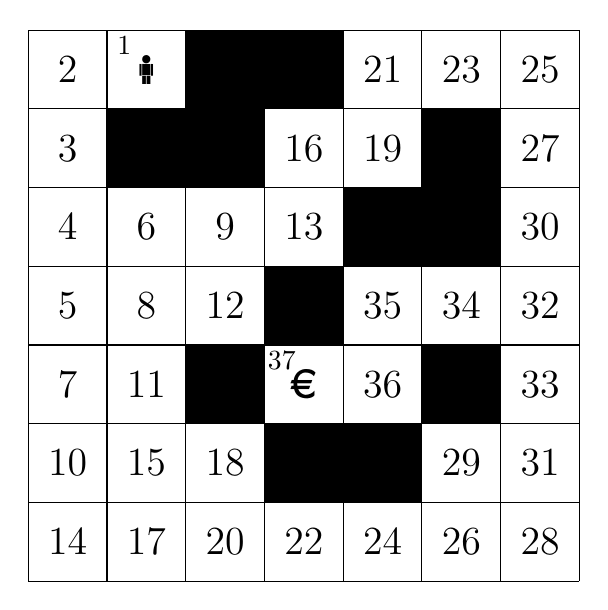
\begin{tikzpicture}
    \draw (0,0) grid (7, 7);
   
    \fill (2, 7) rectangle (4, 6);
    \fill (1, 6) rectangle (2, 5);
    \fill (2, 7) rectangle (3, 5);
    \fill (4, 5) rectangle (6, 4);
    \fill (5, 6) rectangle (6, 4);
    \fill (3, 4) rectangle (4, 3);
    \fill (2, 3) rectangle (3, 2);
    \fill (3, 2) rectangle (5, 1);
    \fill (5, 2) rectangle (6, 3);
    
    \node at (1.5, 6.5) {\Large \Gentsroom};
    \node at (3.5, 2.5) {\Large \EURhv};

    % Begin
    \node at (0.5, 0.5) {\Large 14};
    \node at (1.5, 0.5) {\Large 17};
    \node at (2.5, 0.5) {\Large 20};
    \node at (3.5, 0.5) {\Large 22};
    \node at (4.5, 0.5) {\Large 24};
    \node at (5.5, 0.5) {\Large 26};
    \node at (6.5, 0.5) {\Large 28};
    \node at (0.5, 1.5) {\Large 10};
    \node at (1.5, 1.5) {\Large 15};
    \node at (2.5, 1.5) {\Large 18};
    % \node at (3.5, 1.5) {\Large 24}; WALL
    % \node at (4.5, 1.5) {\Large 24}; WALL
    \node at (5.5, 1.5) {\Large 29};
    \node at (6.5, 1.5) {\Large 31};
    \node at (0.5, 2.5) {\Large 7};
    \node at (1.5, 2.5) {\Large 11};
    % \node at (2.5, 2.5) {\Large 34}; WALL
    \node at (3.22, 2.8) {\normalsize 37}; % GOAL
    \node at (4.5, 2.5) {\Large 36};
    %\node at (5.5, 2.5) {\Large }; WALL
    \node at (6.5, 2.5) {\Large 33};
    \node at (0.5, 3.5) {\Large 5};
    \node at (1.5, 3.5) {\Large 8};
    \node at (2.5, 3.5) {\Large 12};
    % \node at (3.5, 3.5) {\Large 24}; WALL
    \node at (4.5, 3.5) {\Large 35};
    \node at (5.5, 3.5) {\Large 34};
    \node at (6.5, 3.5) {\Large 32};
    \node at (0.5, 4.5) {\Large 4};
    \node at (1.5, 4.5) {\Large 6};
    \node at (2.5, 4.5) {\Large 9};
    \node at (3.5, 4.5) {\Large 13};
    % \node at (4.5, 4.5) {\Large 24}; WALL
    % \node at (5.5, 4.5) {\Large 24}; WALL
    \node at (6.5, 4.5) {\Large 30};
    \node at (0.5, 5.5) {\Large 3};
    % \node at (1.5, 5.5) {\Large 24}; WALL
    % \node at (2.5, 5.5) {\Large 24}; WALL
    \node at (3.5, 5.5) {\Large 16};
    \node at (4.5, 5.5) {\Large 19};
    % \node at (5.5, 5.5) {\Large 24}; WALL
    \node at (6.5, 5.5) {\Large 27};
    \node at (0.5, 6.5) {\Large 2};
    \node at (1.22, 6.8) {\normalsize 1}; % PERSON
    % \node at (2.5, 6.5) {\Large 24}; WALL
    % \node at (3.5, 6.5) {\Large 24}; WALL
    \node at (4.5, 6.5) {\Large 21};
    \node at (5.5, 6.5) {\Large 23};
    \node at (6.5, 6.5) {\Large 25};
    % End
\end{tikzpicture}
}
\end{center}
\end{answers}



\begin{enumerate}
\setcounter{enumi}{2}
\item Show on the right maze the board positions visited by $A^{\star}$ graph search with a manhattan distance heuristic (ignoring walls), by writing the order numbers in the relevant cells. A state is visited when it is selected in the fringe and expanded. When several states have the smallest path cost, they are visited in the same lexicographical order as the one used for uniform-cost graph search. \textbf{(1 pt)}
\end{enumerate}

\begin{answers}[5.2cm]
% Your answer here
\begin{center}
\resizebox{5cm}{!}{
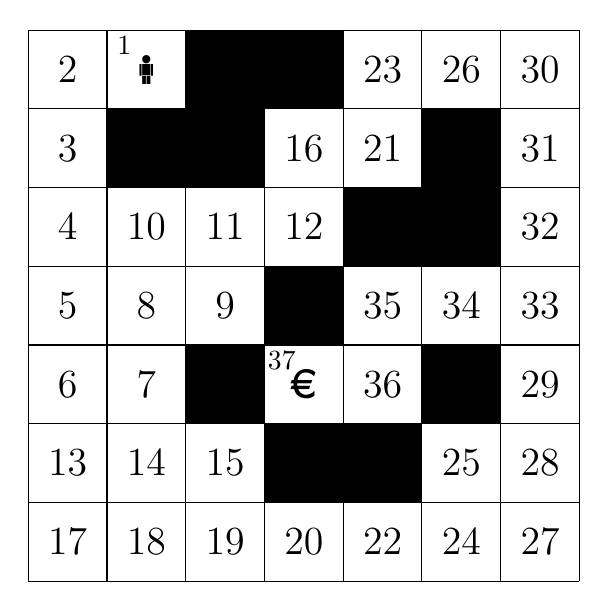
\begin{tikzpicture}
    \draw (0,0) grid (7, 7);
   
    \fill (2, 7) rectangle (4, 6);
    \fill (1, 6) rectangle (2, 5);
    \fill (2, 7) rectangle (3, 5);
    \fill (4, 5) rectangle (6, 4);
    \fill (5, 6) rectangle (6, 4);
    \fill (3, 4) rectangle (4, 3);
    \fill (2, 3) rectangle (3, 2);
    \fill (3, 2) rectangle (5, 1);
    \fill (5, 2) rectangle (6, 3);
      
    \node at (1.5, 6.5) {\Large \Gentsroom};
    \node at (3.5, 2.5) {\Large \EURhv};

    % Begin
    % J'avais ça avant
    % \node at (0.5, 0.5) {\Large 20};
    % \node at (1.5, 0.5) {\Large 17};
    % \node at (2.5, 0.5) {\Large 18};
    % \node at (3.5, 0.5) {\Large 19};
    \node at (0.5, 0.5) {\Large 17};
    \node at (1.5, 0.5) {\Large 18};
    \node at (2.5, 0.5) {\Large 19};
    \node at (3.5, 0.5) {\Large 20};
    \node at (4.5, 0.5) {\Large 22};
    \node at (5.5, 0.5) {\Large 24};
    \node at (6.5, 0.5) {\Large 27};
    \node at (0.5, 1.5) {\Large 13};
    \node at (1.5, 1.5) {\Large 14};
    \node at (2.5, 1.5) {\Large 15};
    % \node at (3.5, 1.5) {\Large 24}; WALL
    % \node at (4.5, 1.5) {\Large 24}; WALL
    \node at (5.5, 1.5) {\Large 25};
    \node at (6.5, 1.5) {\Large 28};
    \node at (0.5, 2.5) {\Large 6};
    \node at (1.5, 2.5) {\Large 7};
    % \node at (2.5, 2.5) {\Large 34}; WALL
    \node at (3.22, 2.8) {\normalsize 37}; % GOAL
    \node at (4.5, 2.5) {\Large 36};
    %\node at (5.5, 2.5) {\Large }; WALL
    \node at (6.5, 2.5) {\Large 29};
    \node at (0.5, 3.5) {\Large 5};
    \node at (1.5, 3.5) {\Large 8};
    \node at (2.5, 3.5) {\Large 9};
    % \node at (3.5, 3.5) {\Large 24}; WALL
    \node at (4.5, 3.5) {\Large 35};
    \node at (5.5, 3.5) {\Large 34};
    \node at (6.5, 3.5) {\Large 33};
    \node at (0.5, 4.5) {\Large 4};
    \node at (1.5, 4.5) {\Large 10};
    \node at (2.5, 4.5) {\Large 11};
    \node at (3.5, 4.5) {\Large 12};
    % \node at (4.5, 4.5) {\Large 24}; WALL
    % \node at (5.5, 4.5) {\Large 24}; WALL
    \node at (6.5, 4.5) {\Large 32};
    \node at (0.5, 5.5) {\Large 3};
    % \node at (1.5, 5.5) {\Large 24}; WALL
    % \node at (2.5, 5.5) {\Large 24}; WALL
    \node at (3.5, 5.5) {\Large 16};
    \node at (4.5, 5.5) {\Large 21};
    % \node at (5.5, 5.5) {\Large 24}; WALL
    \node at (6.5, 5.5) {\Large 31};
    \node at (0.5, 6.5) {\Large 2};
    \node at (1.22, 6.8) {\normalsize 1}; % PERSON
    % \node at (2.5, 6.5) {\Large 24}; WALL
    % \node at (3.5, 6.5) {\Large 24}; WALL
    \node at (4.5, 6.5) {\Large 23};
    \node at (5.5, 6.5) {\Large 26};
    \node at (6.5, 6.5) {\Large 30};
    % End
\end{tikzpicture}
}
\end{center}
\end{answers}




\section{N-Amazons problem (8 pts)}

\begin{enumerate}
  \item Model the N problem as a search problem; describe: \textbf{(2 pts)}
		\begin{itemize}
			\item States
			\item Initial state
			\item Actions / Transition model
			\item Goal test
			\item Path cost function
		\end{itemize}
\end{enumerate}

\begin{answers}[8cm]
\small{$\bullet$ A \textbf{\textit{state}} can be represented as an N x N grid, where each square can either be occupied by an Amazon (symbolized by 'A') or be empty (symbolized by $'\#'$). While this method is intuitive, it requires storing $N^2$ elements in memory for each state. A more efficient approach is to represent a state as a list of N elements, where each index corresponds to a column and the value associated with that index represents the row where an Amazon is placed in that column. A value of -1 indicates that no Amazon is placed in that column. \\
$\bullet$ The \textbf{\textit{initial state}} is a list of N elements initialised to -1 because there are initially no Amazons on the board. \\
$\bullet$ \textbf{\textit{Actions}} involve placing an Amazon in the first empty column of the grid, ensuring that the Amazon is positioned in a square where no attacks occur. In other words, an action entails placing an integer between 0 and N - 1 in the first index of the list where the current value is -1. Only integers that avoid conflicts between Amazons are considered as valid actions. An attack conflict arises when one Amazon threatens another, indicating they share the same row, column (impossible with the Problem modeling), diagonal, or occupy specific squares on the board. These squares correspond to the extended knight's moves: either 3 tiles in one direction followed by 2 tiles in another, or 4 tiles in one direction followed by 1 tile in another. \\
$\bullet$ The \textbf{\textit{transition model}} entails placing the row index (specified by the action) representing a new Amazon into the first element of the list where the value is currently equal to -1. \\
$\bullet$ The \textbf{\textit{goal test}} involves checking if the last element of the list contains an integer between 0 and N - 1 (different of -1). If so, it means that all Amazons have been placed on the board. \\
$\bullet$ The \textbf{\textit{path cost function}} can be defined as the total number of Amazons placed on the board. Each placement of an Amazon incurs a unit cost, and the total path cost is the sum of these individual placement costs. The \textbf{optimal cost} is thus \textbf{N}.}
\end{answers}


\newpage
\begin{enumerate}
\setcounter{enumi}{1}
\item Give an upper bound on the number of different states for an N-Amazons problem with N=n. Justify your answer precisely. \textbf{(0.5 pt)}
\end{enumerate}

\begin{answers}[5cm]
\small{To calculate the total number of possible configurations for the N-Amazons problem on a board of \textbf{size n x n}, we consider that each Amazon \textbf{can be placed in any of the n rows for each column, without any restrictions}. In other words, we do not take into account the constraint that there can be no attack conflicts between the Amazons placed on the board.
Hence, the \textbf{total number of possible configurations} is simply \textbf{$n^n$}, as \textbf{for each column}, there are \textbf{n available squares to place an Amazon}. The more mathematical explanation is as follows. The formula $n^n$ represents a form of permutation, where each element \textbf{can be chosen from n possible choices, and this is repeated n times}. This formula is used in the context of \textbf{arrangements with repetition}. \textbf{Another upper bound} that is more precise is \textbf{n!}, as we know that the \textbf{Amazons cannot be placed in the same row}. Once an Amazon is placed in a row, that row cannot be used again. Therefore, for the first action, there are n possibilities, then n-1 possibilities, n-2, and so on. Hence, a more precise upper bound is indeed n!. To find these upper bounds, I \textbf{relax the problem} (remove a constraint). \textbf{\textit{The more we relax the problem, the less precise the upper bound becomes}}.}

\end{answers}



\begin{enumerate}
\setcounter{enumi}{2}
\item Give an admissible heuristic for a N=n. Prove that it is admissible. What is its complexity ? \textbf{(1 pts)}
\end{enumerate}

\begin{answers}[5cm]
\footnotesize{I have opted for a \textbf{\textit{heuristic}} that minimizes conflicts between each already placed Amazon on the chessboard and the empty tiles in the remaining columns (= empty columns). For each attack by an Amazon, the \textit{heuristic} score is incremented by 1. Hence, this \textit{heuristic} effectively represents the number of tiles that are under attack by the already placed Amazons, making it impossible to place a new Amazon on those tiles. It's important to note that a single tile can be attacked by multiple Amazons, resulting in multiple conflicts for that tile. Moreover, this heuristic doesn't take into account the conflicts between each Amazon already placed because, by construction of the problem, each action consist to place a new Amazon without creating a conflict (see question \textit{2.1}).

This \textit{heuristic} is \textbf{\textit{admissible}} because its \textbf{minimum score is 0 and is only reached when all the columns are filled}. \textbf{As soon as a column is not filled, the \textit{heuristic} score is greater than 0} because there is at least $n - 1$ conflicts since two Amazons cannot be on the same row, demonstrating that the \textbf{\textit{heuristic} never overestimates the cost to reach a goal state}. Thus, this \textit{heuristic} is indeed \textbf{\textit{admissible}}.

The time complexity of this \textit{heuristic} is $\mathcal{O}(x*(n-x)*n)$, where \textbf{x} is the \textbf{number of Amazons already placed on the chessboard} and \textbf{n} is \textbf{the size of the chessboard}. An \textbf{upper bound} on this complexity is therefore $\mathcal{O}(n^3)$.}
\end{answers}

\begin{enumerate}
\setcounter{enumi}{4}
\item \textbf{Implement} your solver. Extend the \emph{Problem} class and implement 
		the necessary methods and other class(es) if necessary.  \textbf{(0.5 pt)}
\item \textbf{Experiment}, compare and analyze informed (\emph{astar\_graph\_search}), uninformed \\
    (\emph{breadth\_first\_graph\_search} and \emph{depth\_first\_graph\_search}) graph search of aima-python3 on N = [10, 11, 12, 13, 20, 25, 30]. \textbf{(3 pts for the whole question)}
		
		Report in a table the time and the number of explored nodes and the number of 
		steps to reach the solution.
		
		Are the number of explored nodes always smaller with 
		\emph{astar\_graph\_search}? 
		What about the computation time? 
		Why? 
		 
		 When no solution can be found by a strategy in a reasonable time (say \textbf{3 
		 min}), indicate the reason (time-out and/or exceeded the memory).
\end{enumerate}

\begin{answers}[8cm]
\small{Firstly, it's noticeable that the \textbf{number of steps} is equivalent to the \textbf{size of the chessboard for all searches}, which is expected due to the construction of the problem discussed in question \textit{2.1}.

Next, it can be observed that the \textbf{\textit{execution time}} of A* is significantly \textbf{smaller} compared to algorithms like BFS\_graph or DFS\_graph. The reason for this is that \textbf{A* is guided by a heuristic and is therefore an informed search}. It doesn't blindly search the entire search tree like uninformed searches. Since the \textbf{maximum depth of the tree is N} and the \textbf{optimal solution is guaranteed to be at the last depth}, \textbf{DFS\_graph is much faster than BFS\_graph} because it \textbf{searches in depth} and the \textbf{optimal solution is at the last depth of the search tree}. \textbf{BFS\_graph}, on the other hand, \textbf{searches in breadth and explores almost the entire search tree} (except the last layer, where it's not always necessary to search all of this layer). Thus, a breadth-first search is not optimal for this problem. We can also notice that, for small instances (N <= 13), DFS\_graph is slightly faster than A*.

Regarding the number of \textbf{\textit{explored nodes}}, BFS\_graph obviously \textbf{explores the most nodes since it explores the entire tree} (except the last layer where it's not mandatory). Then, \textbf{for small instances} (N=11/12/13), the number of \textbf{nodes explored by A* and DFS\_graph are comparable and small} (slightly better for A*). However, for \textbf{larger chessboards} (N >= 20), \textbf{A* remains very efficient and explores a reasonable number of nodes} while \textbf{DFS\_graph explores a very large number of nodes}.

Overall, A* stands out as the most efficient algorithm in terms of both time and the number of explored nodes, especially as the problem size increases. Its informed search strategy allows it to focus on the \textbf{most promising paths, resulting in faster convergence to the optimal solution}.}
\end{answers}

~ 

\begin{answers}[6.5cm]
\begin{center}
\begin{tabular}{||l||l|l|l||l|l|l||l|l|l||l|l|l||}
\hline
\multirow{3}{*}{Size Probl. (N)} & \multicolumn{3}{c||}{$A^{\star}$ Graph}& \multicolumn{3}{c||}{BFS Graph} & \multicolumn{3}{c||}{DFS Graph}\\
 & NS & T & EN & NS & T & EN & NS & T & EN\\
\hline
10 & 10 & 674.956 \mu s & 25 & 10 & 0.173 s & 2298 & 10 & 3.007 ms & 325 \\
\hline
11 & 11 & 973.473 \mu s & 18 & 11 & 0.886 s & 7149 & 11 & 232.65 \mu s & 24 \\
\hline
12 & 12 & 11.314 ms & 339 & 12 & 8.474 s & 23923 & 12 & 2.123 ms & 173 \\
\hline
13 & 13 & 3.168 ms & 95 & 13 & 105.935 s & 87922 & 13 & 2.295 ms & 107 \\
\hline
20 & 20 & 18.189 ms & 236 & TO & TO & TO & 20 & 1.069 s & 51861 \\
\hline
25 & 25 & 0.159 s & 1488 & TO & TO & TO & 25 & 10.356 s & 319795 \\
\hline
30 & 30 & 0.47 s & 3129 & TO & TO & TO & 30 & 236.313 s & 5149276 \\
\hline
\hline
\end{tabular}\\

~\\
\textbf{NS}: Number of steps — \textbf{T}: Time — \textbf{EN}: Explored nodes - \textbf{TO}: Time Out - \textbf{EM}: Exceeded memory
\end{center}
\end{answers}



\begin{enumerate}
\setcounter{enumi}{5}
\item \textbf{Submit} your program on INGInious, using the \textit{A*} algorithm with your best heuristic(s).
		 Your file must be named \emph{namazon.py}. 
      Your program should be able to, given an integer as argument, return the correct output.
		 Your program must print to the standard output a solution to the N's given in argument for the N-Amazons problem, satisfying the described output format. \textbf{(2 pts)}
\end{enumerate}

\begin{answer}
I followed the instructions and implemented the problem \textbf{using the modeling presented in question \textit{2.1}}. Additionally, I implemented a \textbf{class named \textit{State}}, which takes as arguments a \textbf{list of N elements} representing the chessboard with Amazons on it, as well as the \textbf{index of the first empty column from the left}. This class facilitates the implementation of the \textbf{\textit{str()}} method for \textbf{formatting the output}, as well as the \textbf{\textit{eq(), hash()}}, and \textbf{\textit{lt()}} methods, which are essential for search methods. The heuristic function for \textbf{\textit{A*}} is explained in question \textit{2.3}.
\end{answer}

\section{Local Search: Sudoku Problem (8 pts)}

\begin{enumerate}
    \item Formulate the Sudoku problem as a Local Search problem (problem, cost function, feasible solutions, optimal solutions). \textbf{(2 pts)}
\end{enumerate}

\begin{answer}
\tiny{
$\bullet$ \textbf{\textit{Problem:}} Given a partially filled 9x9 grid (Sudoku puzzle), represented as a list of lists representing a 2D grid where each cell is either filled with a number or with a 0 indicating an empty cell, the objective is to fill in the empty cells such that each row, column, and 3x3 subgrid contains all the digits from 1 to 9 without repetition.

$\bullet$ \textbf{\textit{Cost Function:}} The cost function in this problem is the evaluation of how close a particular state of the Sudoku grid is to the goal state. In other words, it measures the number of conflicts or violations of Sudoku rules present in the grid. This cost function would assign a higher cost to states with more conflicts. An optimal solution is found when the cost evaluated by this function is equal to 0 (when all the rules are adhered to without any violations).

$\bullet$ \textbf{\textit{Feasible Solutions:}} Feasible solutions are grid configurations where all the digits 1 to 9 appear exactly once in each row, column, and 3x3 subgrid, and where initially fixed cells are respected. So it's a grid where all the constraints are adhered to.

$\bullet$ \textbf{\textit{Optimal Solutions:}} The optimal solution to the Sudoku problem is the best feasible solution where the cost evaluated bu the cost function is equal to zero. This corresponds to a completed Sudoku grid where all cells are filled with digits 1 to 9, satisfying all row, column, and subgrid constraints. In this problem, all feasible solutions are also optimal, as we do not consider the number of states to reach the goal or any other selection criteria. In other words, once a solution satisfies all the constraints and rules of Sudoku, it is deemed optimal, regardless of the path taken to achieve it.}
\end{answer}

\begin{enumerate}
    \item You are given a template on Moodle: \url{sudoku.py}. Implement your own simulated annealing algorithm and your own \url{objective\_score} function. Your program will be evaluated in on 15 instances (during 3 minutes each) of which 5 are hidden. We expect you to solve (get the optimal solution) at least 12 out of the 15. \textbf{(6 pt)}
\end{enumerate}

\begin{answer}
% ANY COMMENTS ABOUT YOUR CODE
\scriptsize{First, I set the \textbf{\textit{cooling rate}} to \textbf{0.9999} to \textbf{allow for the maximum number of iterations} to converge towards the optimal solution. Additionally, I created a function that generates a \textbf{set containing initially fixed positions} in the Sudoku grid. I also create a function \textbf{to fill randomly the board} initially to win some time.
For the \textbf{\textit{neighbor generation function}}, I made optimizations to make it more efficient than generating completely random neighbors. Here, \textbf{I randomly choose a cell among those not initially fixed. Then, I select a random number that does not create a conflict. If all numbers result in a conflict, I repeat the process. After 5 iterations, I return a random number in the selected cell}. This strategy helps to \textbf{escape local minima and reach the global minimum, which is 0} for this objective function. With this improvement, my solver performs significantly faster.
Regarding the \textbf{\textit{objective function}}, I count the \textbf{number of empty cells and the number of conflicts} present in the Sudoku, taking into account the initially fixed cells as well.}
\end{answer}
\end{document}